%% ------------------------------------------------------------------------- %%
\chapter{Correlation rules and proposed extension}
\label{cap:proposed-solution}

\noindent A state of the art skin detection method has been recently developed by~\cite{brancati:17}. In this chapter, we review the method and extend it\footnote{All the implementations can be found at \url{https://bitbucket.org/rodrigoadfaria/skin-detector/}.} adding more rules to enforce the constraints and seeking for a better accuracy in terms of false positive rate without hurting the performance of the original method.


%% ------------------------------------------------------------------------- %%
\section{Correlation rules on YCrYCb colormap}
\label{sec:correlation_rules_ycrycb}
The pixels of human skin have a very particular color. They fall into a restricted range of hues and they are not deeply saturated. This phenomenon is due the appearance of skin: formed by a combination of blood (red) and melanin (brown, yellow), which leads the human skin color to be clustered within a small area in the color space~\citep{fleck:96}.

Although this cluster can be seen in different color spaces, authors often use those where it is possible to split the chrominance from the luminance information. YCbCr is one of these color spaces. \citet{chai:99}~firstly observed this cluster within this particular color space (see Fig.~\ref{fig:dataset_sfa_ycbcr}). Based on a given set of training images, they~\citep{chai:99} built a skin color map using a histogram approach. In this map, the Cr and Cb distributions of skin color fall into the ranges [133, 173] and [77, 127], respectively, regardless the skin color variation in different races (see Fig.~\ref{fig:dataset_sfa_ycbcr_hist}).

\begin{figure}[!ht]
    \centering
    \begin{minipage}{0.485\textwidth}
        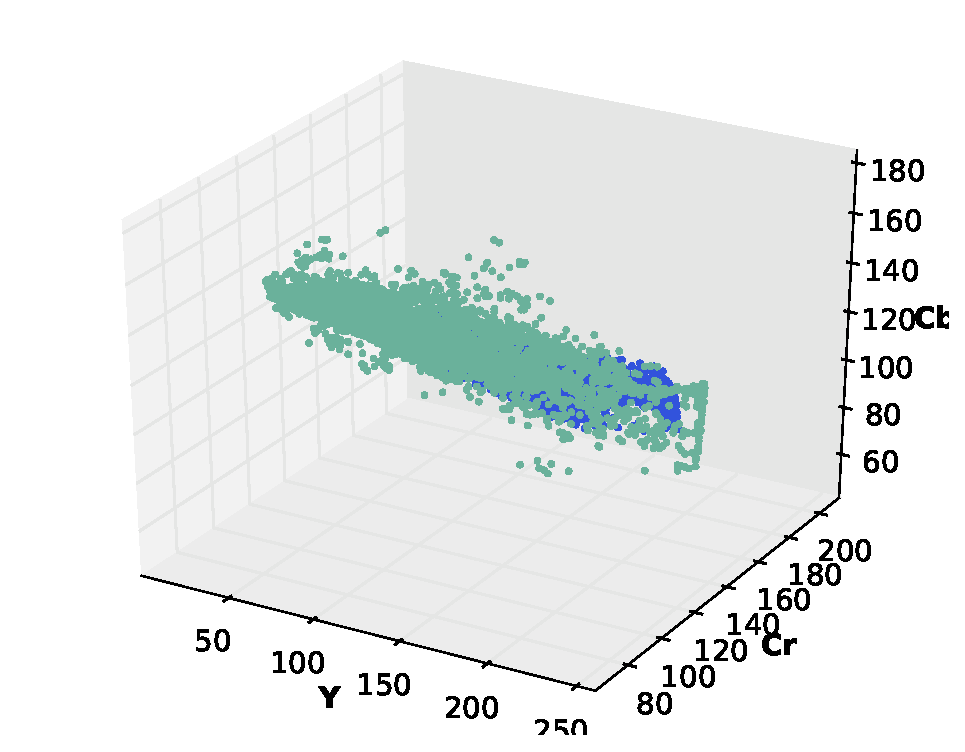
\includegraphics[width=\textwidth]{sfa/sfa_ycbcr}
    \end{minipage}
    ~ % space
    \begin{minipage}{0.485\textwidth}
        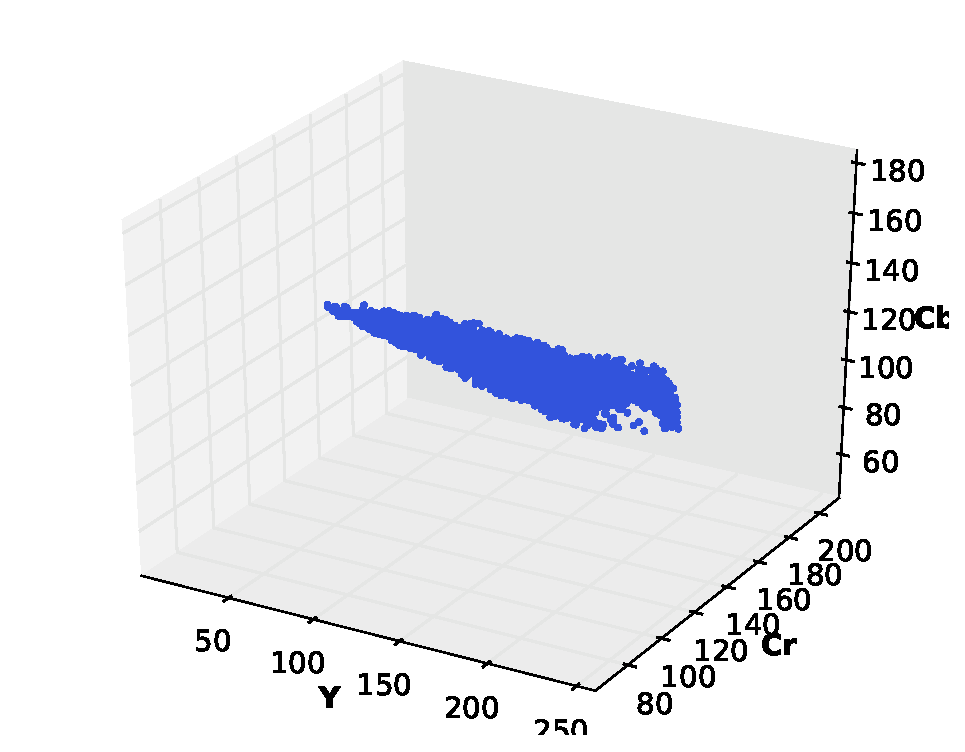
\includegraphics[width=\textwidth]{sfa/sfa_ycbcr_skin_only}
    \end{minipage}
    \caption[3-dimensional view of the YCbCr channels of some image patches of the SFA dataset]{3-dimensional view of the YCbCr channels of some image patches of the SFA dataset. We used the patches with skin samples of size $15 \times 15$. The blue points are skin samples and the green ones are non-skin. On the right (skin samples only), we can clearly see a narrow and thin cluster. Source: adapted from~\citet{chai:99}.}
    \label{fig:dataset_sfa_ycbcr}
\end{figure}

\begin{figure}[!ht]
    \centering
    \begin{minipage}{0.485\textwidth}
        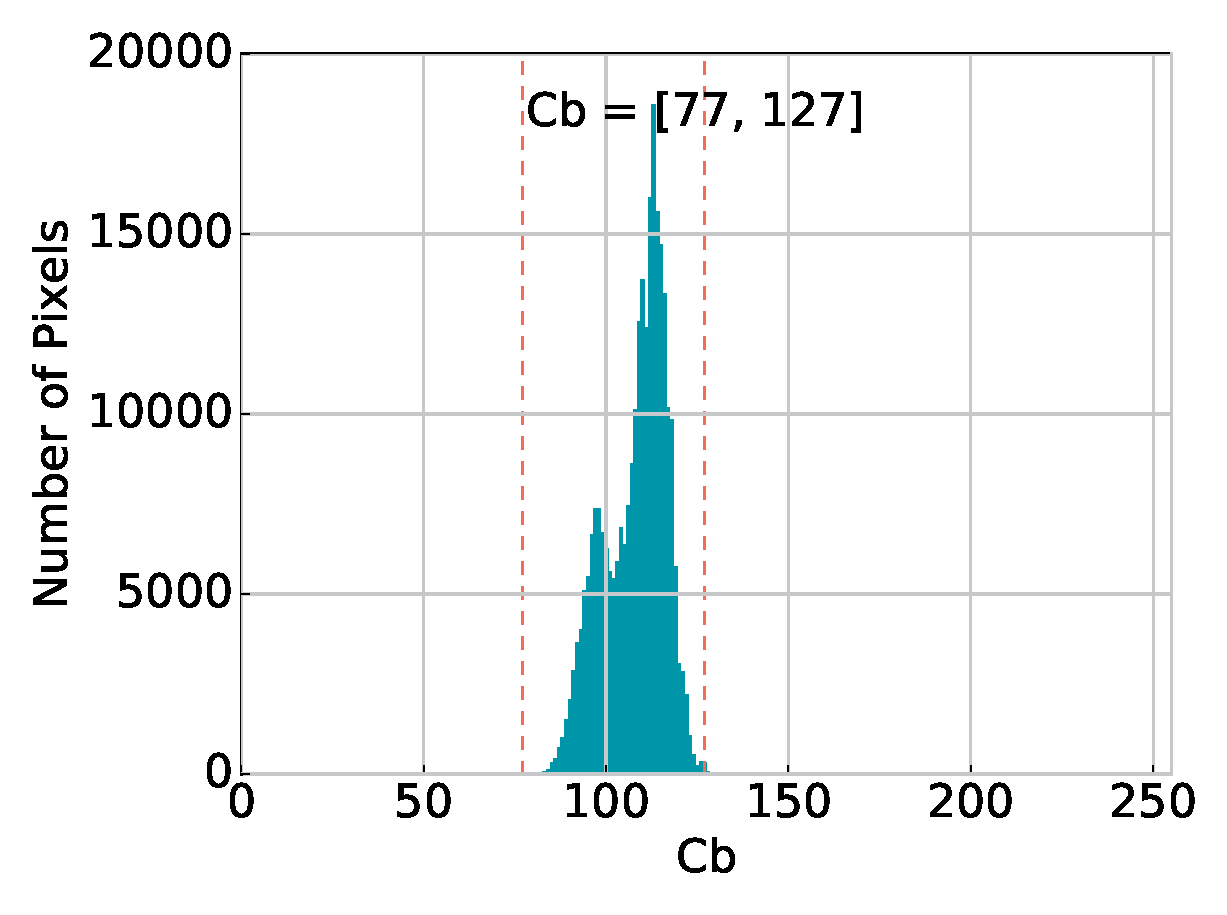
\includegraphics[width=\textwidth]{sfa/sfa_cb_histogram}
    \end{minipage}
    ~ % space
    \begin{minipage}{0.485\textwidth}
        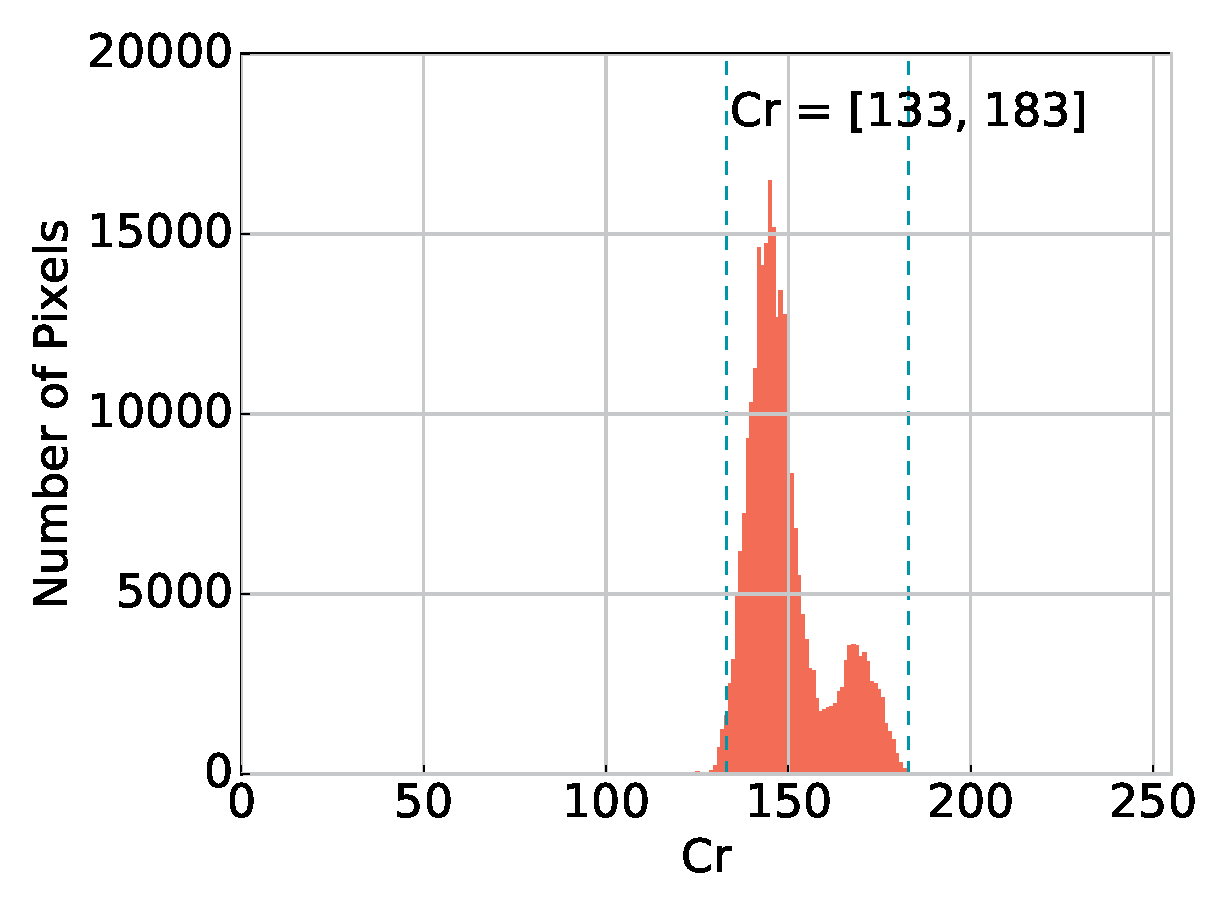
\includegraphics[width=\textwidth]{sfa/sfa_cr_histogram}
    \end{minipage}
    \caption[Histogram of Cb and Cr channels of some image patches of the SFA dataset]{Histogram of Cb and Cr channels of some image patches of the SFA dataset. We used the patches skin samples of size $15 \times 15$. Clearly, the samples (pixels) fall into the intervals observed by~\citet{chai:99}. Source: adapted from~\citet{chai:99}.}
    \label{fig:dataset_sfa_ycbcr_hist}
\end{figure}

Therefore, a very simple and practical approach to detect human skin pixels would be to create a set of rules, based in those ranges, that identify the presence of chrominance (Cr, Cb) values who fit into the rules. In fact, this was the approach used by~\citet{chai:99}.

Another important finding regarding the skin color clusters in the YCbCr color space is their behavior when looking for the compositions of YCb and YCr separately. In other words, where rely this distribution into the YCb and YCr subspaces. In Figure~\ref{fig:obama_trapezoids}, we can see the distribution (clusters) for an image of the Pratheepan dataset. We can clearly see their shapes as taking a trapezoidal form~\citep{hsu:02}.

In fact, the skin color pixels distribution in the YCb and YCr subspaces is a pattern. However, this trapezoidal shape and size will change according to many factors. \citet{brancati:17} observed that change and identified that they are caused mainly due illumination conditions (i.e. the lighting of the scene when the image was acquired influences the size, height, and position of these trapezoidal shape). Moreover, they~\citep{brancati:17} observed an inversely proportional behavior of the chrominance components (Cr, Cb) that could be fitted into a model for skin pixels detection. We will explain in details how this model has been created in Section~\ref{sec:original_method}.

\begin{figure*}[!htb]
    \centering
    \begin{subfigure}[t]{0.48\textwidth}
        \includegraphics[width=\textwidth]{pra/ori/obama}
        \caption{}
    \end{subfigure}
    \begin{subfigure}[t]{0.48\textwidth}
        \includegraphics[width=\textwidth]{pra/gtc/obama}
        \caption{}
    \end{subfigure}
    \begin{subfigure}[t]{0.88\textwidth}
        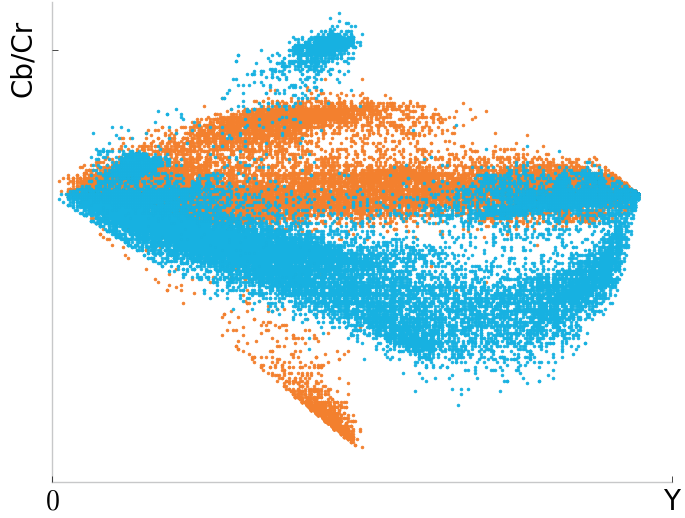
\includegraphics[width=\textwidth]{image_trap_plot}
        \caption{}
    \end{subfigure}

    \caption[Skin pixels distribution in the YCr and YCb subspaces of a sample image]{Skin pixels distribution in the YCr and YCb subspaces of a sample image. Each image is, respectively, (a) sample image from Pratheepan (b) ground truth (c) skin pixels distribution in YCr (orange) and YCb (blue) subspaces. We can clearly see a trapezoidal shape of the pixels distribution. These trapezoids are inversely positioned reflecting the inversely proportional behavior of the chrominance components (Cr, Cb). Source: adapted from~\citet{brancati:17}.}
    \label{fig:obama_trapezoids}
\end{figure*}

%% ------------------------------------------------------------------------- %%
\section{Original method}
\label{sec:original_method}
In order to describe the proposed extensions, we will first present the original method that is based on the definition of image-specific trapezoids, named $T_{YCb}$ and $T_{YCr}$, in the \textit{YCb} and \textit{YCr} subspaces, respectively. The trapezoids are essential to verify a relationship between the chrominance components $Cb$ and $Cr$ in these subspaces~\citep{brancati:17}.

\begin{figure}[ht]
    \centering
    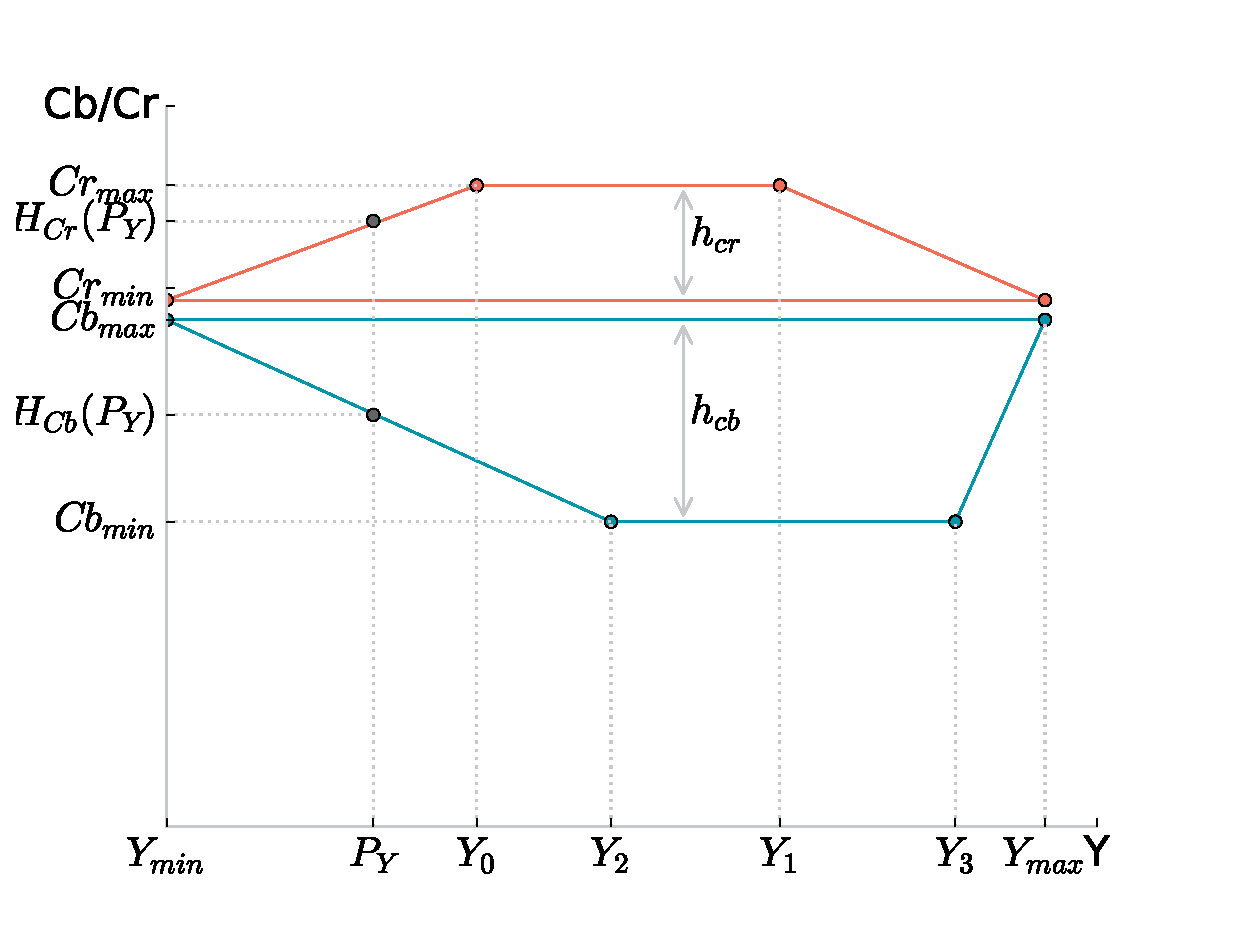
\includegraphics[width=0.8\textwidth]{trapezoids}
    \caption[Graphical representation of the trapezoids as well as their parameters]{Graphical representation of the trapezoids as well as the parameters $Y_{min} = 0$, $Y_{max} = 255$, $Y_{0}$, $Y_{1}$, $Y_{2}$, $Y_{3}$, $Cr_{min}$, $Cr_{max}$, $Cb_{min}$, $Cb_{max}$, $h_{Cr}$, $h_{Cb}$, $H_{Cr}(P_Y)$, $H_{Cb}(P_Y)$. Source: adapted from~\citep{brancati:17}.}
    \label{fig:trapezoids}
\end{figure}

To show the correlations, Brancati et. al. present the YCbCr space as a 2D graph where the $Y$ is presented in the abscissa and the $Cr$ and $Cb$ components is in the ordinate (see Fig.~\ref{fig:trapezoids}). The base of the trapezoids $T_{YCr}$ and $T_{YCb}$ are given by the coordinates $(Y_{min}, Cr_{min})$ and $(Y_{min}, Cb_{max})$ in the $YCr$ and $YCb$ , respectively~\citep{brancati:17}. The values $Cr_{min}$ = 133, $Cb_{max}$ = 128 were selected according to~\citet{chai:99} where a skin color map was designed using a histogram approach based on a given set of training images. Chai and Ngan observed that the Cr and Cb distributions of skin color fall in the ranges [133, 173] and [77, 127], respectively, regardless of the skin color variation in different races (see details in Section~\ref{sec:correlation_rules_ycrycb}).

The $Cr_{max}$ parameter is calculated dynamically, taking into account the histogram of the pixels with $Cr$ values in the range $[Cr_{min}, 183]$, looking for the maximum value of $Cr$ associated with at least 0.1\% \footnote{In \citet{brancati:17} this rate is reported to be equal to 10\%. However, in the distributed source code we found the value 0.1\%, that we are using in the experiments.} of pixels in the image. The same applies to $Cb_{min}$, taking the histogram with $Cb$ values in the range $[77, Cb_{max}]$. $Y_0$ and $Y_1$ (shorter base of the upper trapezoid) are, respectively, the 5${th}$ and 95$th$ percentile of the luminance values associated with the pixels of the image with $Cr = Cr_{max}$~\citep{brancati:17}. A similar procedure is used to find the values of the shorter base of the other trapezoid, $Y_2$ and $Y_3$ (see Fig.~\ref{fig:crmax_computation} for an example).

\begin{figure}[ht]
    \centering
    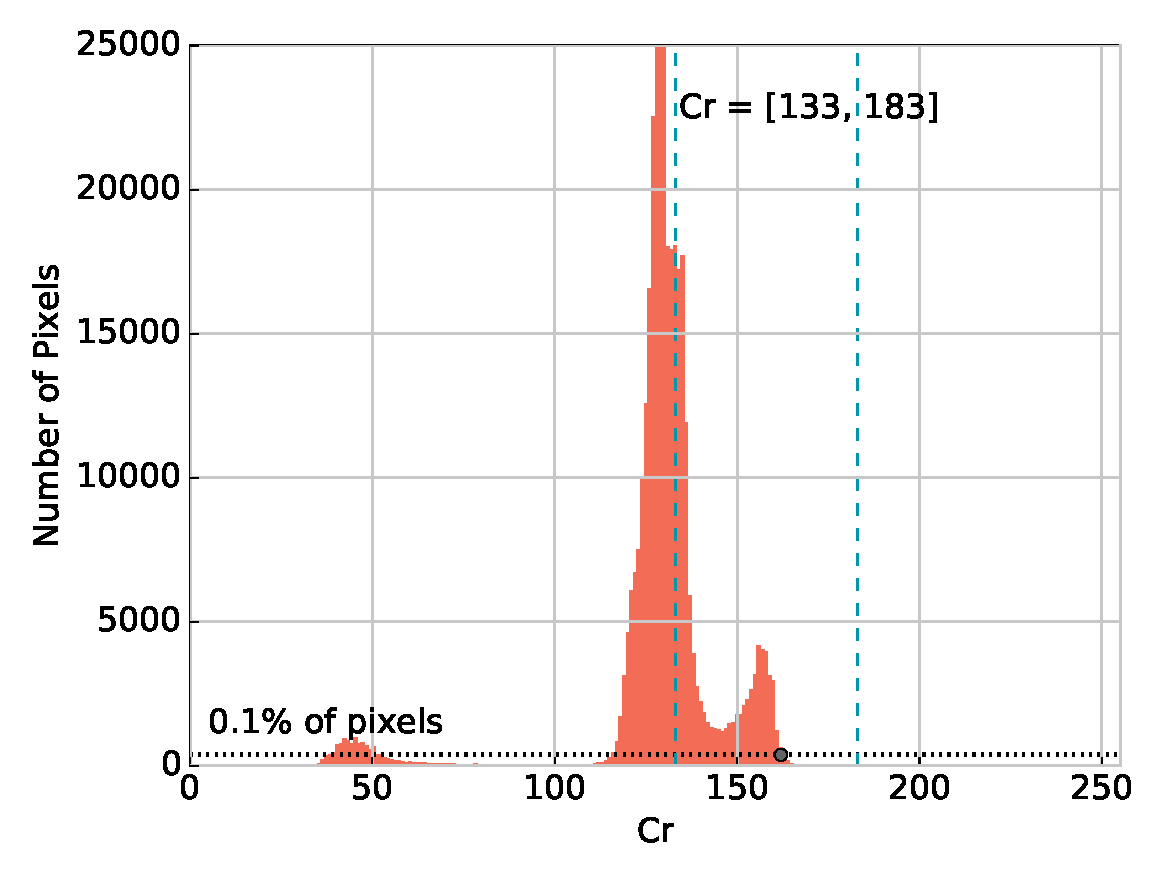
\includegraphics[width=0.7\textwidth]{crmax_computation}
    \caption[Computation of $Cr_{max}$ based on $Cr$ values histogram of a 724 x 526 image]{Computation of $Cr_{max} = 162$ based on $Cr$ values histogram of a 724 x 526 image. Source: adapted from~\citep{brancati:17}.}
    \label{fig:crmax_computation}
\end{figure}

The correlation rules' parameters between the chrominance components $P_{Cr}$ and $P_{Cb}$ of a pixel $P$ are specified as~\citep{brancati:17}:
\begin{itemize}
    \item the minimum difference between the values $P_{Cr}$ and $P_{Cb}$, denoted $I_P$;
    \item an estimated value of $P_{Cb}$, namely $P_{Cb_s}$;
    \item the maximum distance between the points $(P_Y, P_{Cb})$ and $(P_Y, P_{Cb_s})$, denoted $J_P$.
\end{itemize}

Therefore, to determine if $P$ is skin, the following correlation rules, expressed in terms of equations, must hold~\citep{brancati:17}:
\begin{equation}
    P_{Cr} - P_{Cb} \geq I_P
\label{condition_c0}
\end{equation}
\begin{equation}
   |P_{Cb} - P_{Cb_s}| \leq J_P
\label{condition_c1}
\end{equation}

The estimated value $P_{Cb_{s}}$ is given by \footnote{$dP_{Cb_{s}}$ is the distance between the points $(P_Y, P_{Cb_{s}})$ and $(P_Y, Cb_{max})$ in the $YCb$ subspace, calculated on the basis of $dP_{Cr}$, observing the inversely proportional behavior of the components. $\alpha$ is the rate between the normalized heights of the trapezoids in relation to the $P_Y$ value~\citep{brancati:17}.}:
\begin{equation}
    P_{Cb_s} = Cb_{max} - dP_{Cb_s}
\end{equation}
where \footnote{$dP_{Cr}$ is the distance between $(P_Y, P_{Cr})$ and $(P_Y, Cr_{min})$ points in the $YCr$ subspace~\citep{brancati:17}.}:
\begin{align}
    dP_{Cb_s} &= \alpha \cdot dP_{Cr}
    \\
    dP_{Cr} &= P_{Cr} - Cr_{min}
\end{align}

The coordinates of the other sides of the trapezoids are given by $[P_Y, H_{Cr}(P_Y)]$ and $[P_Y, H_{Cb}(P_Y)]$, such that~\citep{brancati:17}:
\begin{align}
  H_{Cr}(Y) &=  \begin{cases}
                Cr_{min} + h_{Cr}\big(\frac{Y - Y_{min}}{Y_0 - Y_{min}}\big) & Y \in [Y_{min},\ Y_0] \\
                Cr_{max} & Y \in [Y_0,\ Y_1] \\
                Cr_{min} + h_{Cr}\big(\frac{Y - Y_{max}}{Y_1 - Y_{max}}\big) & Y \in [Y_1,\ Y_{max}]
              \end{cases}
\\
  H_{Cb}(Y) &=  \begin{cases}
                Cb_{min} + h_{Cb}\big(\frac{Y - Y_2}{Y_{min} - Y_2}\big) & Y \in [Y_{min},\ Y_2] \\
                Cb_{min} & Y \in [Y_2,\ Y_3] \\
                Cb_{min} + h_{Cb}\big(\frac{Y - Y_3}{Y_{max} - Y_3}\big) & Y \in [Y_3,\ Y_{max}]
              \end{cases}
\end{align}

\noindent where $h_{Cr} = Cr_{max} - Cr_{min}$ and $h_{Cb} = Cb_{max} - Cb_{min}$, which are the heights of $T_{YCr}$ and $T_{YCb}$, respectively.

The computation of those points are useful for the calculation of $\alpha$. We first compute the distances $\Delta_{Cr}(P_Y)$ and $\Delta_{Cb}(P_Y)$ between the points $(P_Y, H_{Cr}(P_Y))$, $(P_Y, H_{Cb}(P_Y))$ and the base of the trapezoids~\citep{brancati:17}:
\begin{align}
    \Delta_{Cr}(P_Y) &= H_{Cr}(P_Y) - Cr_{min} \\
    \Delta_{Cb}(P_Y) &= Cb_{max} - H_{Cb}(P_Y)
\end{align}

Next, the distances are normalized with respect to the difference in size of the trapezoids \citep{brancati:17}:
\begin{align}
  \Delta^{'}_{Cr}(P_Y) &=  \begin{cases}
                \Delta_{Cr}(P_Y) \cdot \frac{A_{T_{YCb}}} {A_{T_{YCr}}} &\quad \text{if}\ A_{T_{YCr}} \geq A_{T_{YCb}} \\
                \Delta_{Cr}(P_Y) &\quad \text{otherwise}
              \end{cases}
\\
  \Delta^{'}_{Cb}(P_Y) &=  \begin{cases}
                \Delta_{Cb}(P_Y) &\quad \text{if}\ A_{T_{YCr}} \geq A_{T_{YCb}} \\
                \Delta_{Cb}(P_Y) \cdot \frac{A_{T_{YCr}}} {A_{T_{YCb}}} &\quad \text{otherwise}
              \end{cases}
\end{align}
where $A_{T_{YCr}}$ and $A_{T_{YCb}}$ are the areas of trapezoid ${T_{YCr}}$ and ${T_{YCb}}$, respectively.

Then, the value of $\alpha$ is given by~\citep{brancati:17}:
\begin{equation}
    \alpha = \frac{\Delta^{'}_{Cb}(P_Y)} {\Delta^{'}_{Cr}(P_Y)}
\end{equation}

Finally, $I_P$ \footnote{There is a difference between the source code and the equation that defines $I_P$ in~\citet{brancati:17}. Basically, part of the equation must be taken its absolute value, which we have fixed here.} and $J_P$ are given by~\citep{brancati:17}:
\begin{equation}
    I_P = sf \cdot |(\Delta^{'}_{Cr}(P_Y) - dP_{Cr}) + (\Delta^{'}_{Cb}(P_Y) - dP_{Cb_s})|
    \label{eq:ip}
\end{equation}
\begin{equation}
    J_P = dP_{Cb_s} \cdot \frac{dP_{Cb_s} + dP_{Cr}} {\Delta^{'}_{Cb}(P_Y) + \Delta^{'}_{Cr}(P_Y)}
    \label{eq:jp}
\end{equation}
where:
\begin{equation}
    sf = \frac{min( (Y_1 - Y_0), (Y_3 - Y_2) )} {max( (Y_1 - Y_0), (Y_3 - Y_2) )}
\end{equation}
% Acho que um gráfico mostrando um ponto, ou alguns pontos, no trapézio superior e o respectivo ponto no trapézio inferior seria muito didático. 

%% ------------------------------------------------------------------------- %%
\section{Complementary method}
\label{sec:proposed_method}
The hypothesis assumed in the original method is based on rules that an estimated value of the point $P_{Cb}$, namely $P_{Cb_s}$, must hold in order for the correlation to be valid. On the basis of the inversely proportional behavior of the chrominance components, we will rewrite the correlation rules with respect to the $P_{Cr}$ point.

Thus, we have to refactor the correlation rules' parameters to put them in terms of the estimated value of $P_{Cr}$, that we denote as $P_{Cr_s}$ \footnote{$dP_{Cr_s}$ is the distance between the points $(P_Y, P_{Cr_s})$ and $(P_Y, Cr_{min})$ in the $YCr$ subspace, calculated on the basis of $dP_{Cb}$, observing the inversely proportional behavior of the components. $\alpha$ is the rate between the normalized heights of the trapezoids in relation to the $P_Y$ value.}:
\begin{equation}
    P_{Cr_s} = dP_{Cr_s} + Cr_{min}
\end{equation}
where \footnote{$dP_{Cb}$ is the distance between $(P_Y, P_{Cb})$ and $(P_Y, Cb_{max})$ points in the $YCb$ subspace.}:
\begin{equation}
    dP_{Cr_s} = \alpha \cdot dP_{Cb}
\end{equation}
\begin{equation}
    dP_{Cb}   = Cb_{max} - P_{Cb}
\end{equation}

Next, the constraints given by $I_P$ and $J_P$ in the Eq. \ref{eq:ip} and \ref{eq:jp} respectively, can be redefined as:
\begin{equation}
    I^{'}_P = sf \cdot |(\Delta^{'}_{Cr}(P_Y) - dP_{Cr_s}) + (\Delta^{'}_{Cb}(P_Y) - dP_{Cb})|
\end{equation}
\begin{equation}
    J^{'}_P = dP_{Cr_s} \cdot \frac{dP_{Cb} + dP_{Cr_s}} {\Delta^{'}_{Cb}(P_Y) + \Delta^{'}_{Cr}(P_Y)}
\end{equation}

Therefore, to determine if the pixel $P$ is skin, we have to modify the correlations rules given by Eq. \ref{condition_c0} and \ref{condition_c1}:
\begin{equation}
    P_{Cr} - P_{Cb} \geq I^{'}_P
\label{condition_c00}
\end{equation}
\begin{equation}
   |P_{Cr} - P_{Cr_s}| \leq J^{'}_P
\label{condition_c11}
\end{equation}

Doing this simple extension, we need now to apply the method to the same sets of images to evaluate, in fact, the inversely proportional behavior of the chrominance components. More than that, we can combine all these constraints, given by the pair equations \ref{condition_c0} and \ref{condition_c1}, \ref{condition_c00} and \ref{condition_c11}, to reinforce the firstly defined hypothesis.


\begin{figure}[!htp]
    \centering
    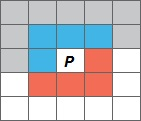
\includegraphics[width=0.25\textwidth]{pixel_neighborhood}
    \caption[Neighbors evaluation with respect to a pixel $P$]{Neighbors evaluation with respect to $P$. If the image is scanned in raster order, $N_8^-(P)$ is the set of points that can be reached before $P$ in an 8-\textit{neighbors} window. In other words, $N_8^-(P)$ are the blue points which we already have evaluated. Source: proposed by the author.}
    \label{fig:pixel_neighborhood}
\end{figure}


%% ------------------------------------------------------------------------- %%
\section{Neighborhood extended method}
\label{sec:neighborhood_extended_method}
Both methods presented in Sections~\ref{sec:original_method} and \ref{sec:proposed_method} can be applied to detect skin pixels, either separated or combined (i.e. the four equations of the correlation rules of each method -- original and complementary -- must hold). However, skin pixels do not usually appear isolated and we could improve the method using some of the already processed neighbors of a pixel $P$, in order to decide if $P$ represents human skin, or not.

To do that, let $N_8^-(P)$ be the 8-\textit{neighbors} of $P$ that can be reached before $P$ when scanning the image in raster order~\citep{rosenfeld:66}. We can see this idea graphically represented by the blue points in Figure~\ref{fig:pixel_neighborhood}.

Thus, we classify $P$ as skin in the following manner: if the constraints given by the pair of equations \ref{condition_c0} and \ref{condition_c1}, as well as \ref{condition_c00} and \ref{condition_c11} hold, then $P$ is classified as skin. When only one of the conditions is satisfied, then we check the decision in $N_8^-(P)$. If three or more pixels are skin, then $P$ will also be classified as a skin pixel. Figure~\ref{fig:n8-flowchart} shows a flowchart of the aforementioned procedure described.

\begin{figure}[ht]
    \centering

    % Define block styles
    \tikzstyle{decision} = [diamond, draw, fill=blue!20,
        text width=4.5em, text badly centered, node distance=3cm, inner sep=0pt]
    \tikzstyle{block} = [rectangle, draw, fill=blue!20,
        text width=5em, text centered, rounded corners, minimum height=4em]
    \tikzstyle{line} = [draw, -latex']
    \tikzstyle{cloud} = [draw, ellipse,fill=red!20, node distance=3cm,
        minimum height=2em]

    \begin{tikzpicture}[node distance = 3cm, auto]
        % Place nodes
        \node [block] (pcrs) {calculate \ref{condition_c00} and \ref{condition_c11} rules};
        \node [block, left of=pcrs] (pcbs) {calculate \ref{condition_c0} and \ref{condition_c1} rules};
        \node [decision, below of=pcrs] (bothtrue) {both true?};
        \node [block, right of=bothtrue, node distance=4cm, fill=gray!20] (isskin) {$P$ is skin};
        \node [decision, below of=bothtrue] (bothfalse) {both false?};
        \node [block, right of=bothfalse, node distance=4cm, fill=gray!20] (noskin) {$P$ is non skin};
        \node [decision, right of=noskin, node distance=4cm] (n8decision) {skin pixels $\geq 3$};
        \node [block, below of=n8decision, node distance=3cm] (n8) {check decision in $N_8^-(P)$};
        % Draw edges
        \path [line] (pcrs) -- (bothtrue);
        \path [line] (bothtrue) -- node {no} (bothfalse);
        \path [line] (bothfalse) -- node {yes} (noskin);
        \path [line] (bothfalse) |- node [near start] {no} (n8);
        \path [line] (bothtrue) -- node {yes}  (isskin);
        \path [line] (n8) -- (n8decision);
        \path [line] (n8decision) |- node [near start] {yes} (isskin);
        \path [line] (n8decision) -- node [near start] {no} (noskin);
        \path [line] (pcbs) |- (bothtrue);
    \end{tikzpicture}

    \caption[Flowchart of our proposed neighbors method]{Flowchart of our proposed neighbors method. In \textbf{both false} decision, the \textbf{no} path means that one of the rules is true and we are in doubt if $P$ is skin or not -- here is where the neighbors are used to find out the label of $P$. Source: proposed by the author.}
    \label{fig:n8-flowchart}
\end{figure}


%% ------------------------------------------------------------------------- %%
\section{Heuristics to fix neighborhood extended method}
\label{sec:sup_neighborhood_operations}
The neighborhood extended method presented in Section~\ref{sec:neighborhood_extended_method} will end up with an undesired behavior on the output images that we called \textit{diagonal effect} (see Fig.~\ref{fig:diagonal_effect}). In addition, besides being visually undesirable, the \textit{diagonal effect} phenomenon causes us to have an increase in the false positive rate. This is caused due to the shape of the window being used. Once we look only for the four already visited pixels of the 8-\textit{neighbors} window, the operation is so based in a non-symmetrical mask. Ideally, we could use another neighborhood strategy and look for all the eight neighbors of the pixel $P$ being evaluated. However, this particular implementation can add extra computational time and affect the performance of the method. 

Therefore, we created an adaptation of the neighborhood method shown in Section~\ref{sec:neighborhood_extended_method}. In this version, we scan the image, with a size of $W \times H$, in the raster order, and apply the original and the extended complementary correlation rules for every single pixel. We keep both results in a matrix of the same size ($W \times H$) of the input image. For each coordinate of this output matrix, we will have a two-position vector with the result of the original and complementary rules answer for this pixel. Next, we read each position of this output matrix and we apply an 8-\textit{neighbors} operations in four different implementations, looking for the majority (five at least) neighbors:

\begin{enumerate}[label={(\arabic*)}]
    \item we look in the correlation rules answer performing an AND. In other words, if both original and complementary correlation rules are saying this pixel is skin, then we classify it as skin;
    \item we look in the correlation rules answer performing an OR. In other words, if one of the correlation rules (original or complementary) is saying this pixel is skin, then we classify it as skin;
    \item we look in the neighbors only querying the original ($P_{Cb_s}$) correlation rules;
    \item we look in the neighbors only querying the complementary ($P_{Cr_s}$) correlation rules.
\end{enumerate}

Of course, this variation will add some additional computational cost once we will scan the image one more time. This implementation can be enhanced, but the idea here is to only explore better the connectivity of the 8-\textit{neighbors} window and check, on the basis of a symmetric mask window, if the \textit{diagonal effect} is gone as well as the measures are improved. Some experiments can be seen further in Section~\ref{sec:sno_experiments}.

\begin{figure*}[!htb]
    \centering
    \begin{subfigure}[t]{0.18\textwidth}
        \includegraphics[width=2.6cm]{sfa/ori/img14}
        \includegraphics[width=2.6cm]{pra/ori/chenhao0017me9}
        \includegraphics[width=2.6cm]{hgr/ori/N_P_hgr1_id04_5}
        \includegraphics[width=2.6cm]{cpq/ori/1923132}
        \includegraphics[width=2.6cm]{cpq/ori/2226882}
        \caption{}
    \end{subfigure}
    \begin{subfigure}[t]{0.18\textwidth}
        \includegraphics[width=2.6cm]{sfa/gt/img14}
        \includegraphics[width=2.6cm]{pra/gt/chenhao0017me9}
        \includegraphics[width=2.6cm]{hgr/gt/N_P_hgr1_id04_5}
        \includegraphics[width=2.6cm]{cpq/gt/1923132}
        \includegraphics[width=2.6cm]{cpq/gt/2226882}
        \caption{}
    \end{subfigure}
    \begin{subfigure}[t]{0.18\textwidth}
        \includegraphics[width=2.6cm]{sfa/cmb/img14}
        \includegraphics[width=2.6cm]{pra/cmb/chenhao0017me9}
        \includegraphics[width=2.6cm]{hgr/cmb/N_P_hgr1_id04_5}
        \includegraphics[width=2.6cm]{cpq/cmb/1923132}
        \includegraphics[width=2.6cm]{cpq/cmb/2226882}
        \caption{}
    \end{subfigure}
    \begin{subfigure}[t]{0.18\textwidth}
        \includegraphics[width=2.6cm]{sfa/ngh/dgn/img14}
        \includegraphics[width=2.6cm]{pra/ngh/dgn/chenhao0017me9}
        \includegraphics[width=2.6cm]{hgr/ngh/dgn/N_P_hgr1_id04_5}
        \includegraphics[width=2.6cm]{cpq/ngh/dgn/1923132}
        \includegraphics[width=2.6cm]{cpq/ngh/dgn/2226882}
        \caption{}
    \end{subfigure}

    \caption[Image samples with the diagonal effect after the neighbors method segmentation]{Image samples with the diagonal effect after the neighbors method segmentation. Each image is from (top-down) SFA, Pratheepan, HGR, and Compaq (latest two) datasets, respectively, where: (a) original image (b) ground truth (c) combined method (f) neighbors method. Independently of the classification accuracy, we can clearly see the diagonal effect present in the output of the neighbors method segmentation in comparison with combined. Besides being a visually undesirable effect, this phenomenon causes us to have an increase in the false positive rate.}
    \label{fig:diagonal_effect}
\end{figure*}